\documentclass[main.tex]{subfiles}

\begin{document}
\section{整体设计}
\subsection{整体设计框图}
系统整体设计如下方框图所示。图中白色方框为模块,橙色梯形为MUX,箭头连线为数据连接线,彩色图形为控制信号。
\begin{figure}[h]
\centering
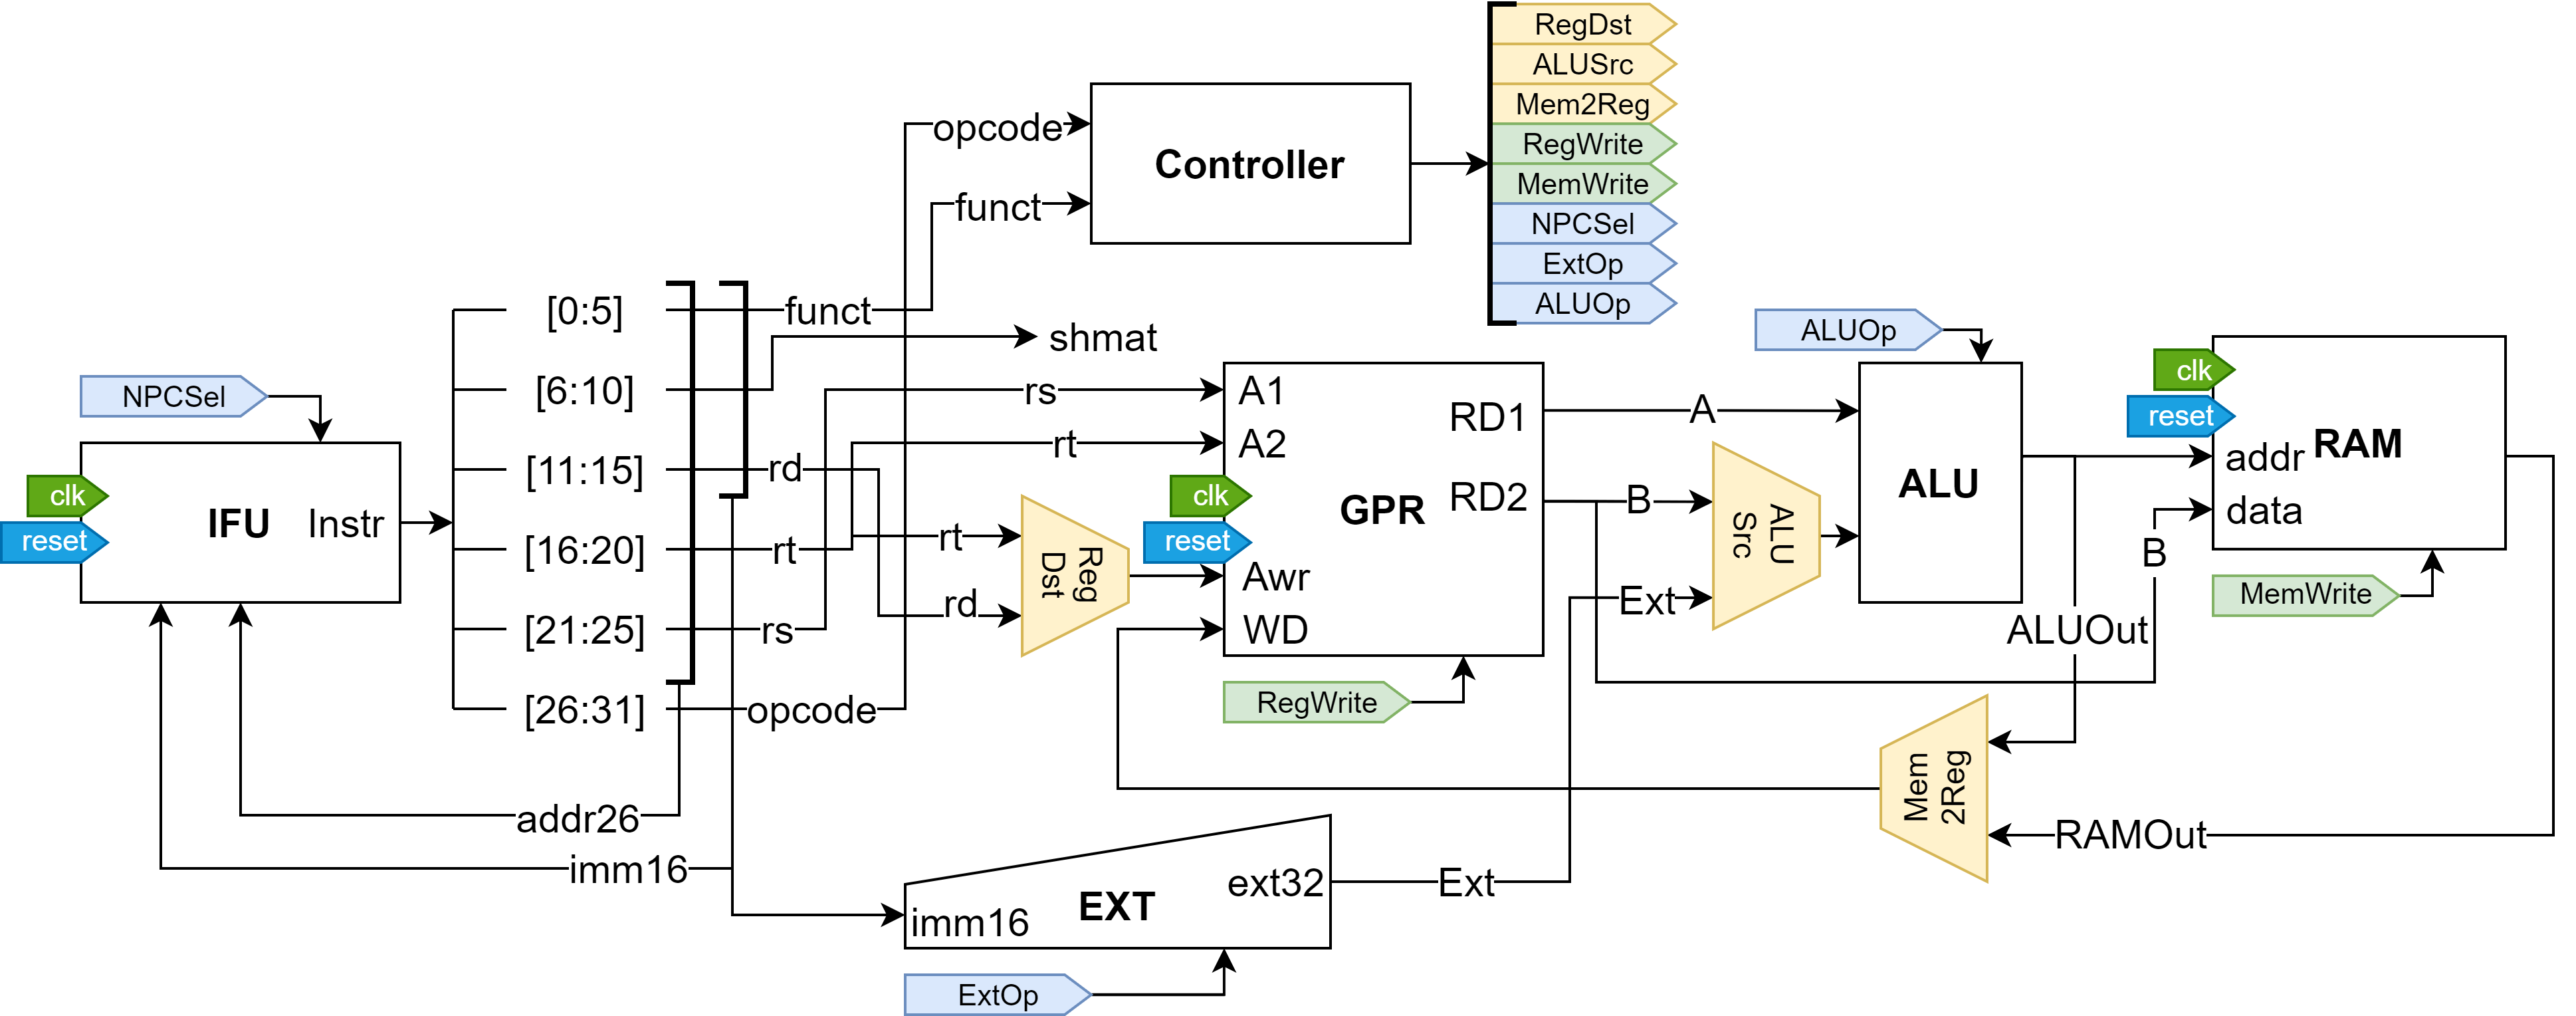
\includegraphics[width=\textwidth]{images/PCOA-overall-block.png}
\caption{整体设计框图}
\end{figure}

图中共有$6$个模块,分别与任务要求的六个模块对应,实现的功能与课程要求一致。

图中共有$8$路控制信号,均由$Controller$模块产生。具体功能见下表。

\begin{center}
    \captionof{table}{控制信号说明}
    \begin{tabular}{c c c c c}
        \toprule
        标识颜色 & 控制信号类型 & 位宽 & 作用元件 & 效果\\
        \midrule
         黄色 & 数据控制信号 & 1bit & 32bit二选一MUX & 从两路信号中选择一路 \\
         绿色 & 写入使能信号 & 1bit & 存储器(寄存器组、内存) & 高有效写入使能 \\
         蓝色 & 模块功能信号 & 2bit & 多功能运算模块 & 选择模块功能 \\
        \bottomrule
    \end{tabular}
\end{center}

图中共有两路外部输入信号:时钟信号$clk$和系统重置信号$reset$。

\clearpage

\subsection{设计框图与电路图对应关系}

整体电路图与设计框图中的模块、信号一一对应。整体电路图(main电路图)如下。

\begin{figure}[h]
\centering
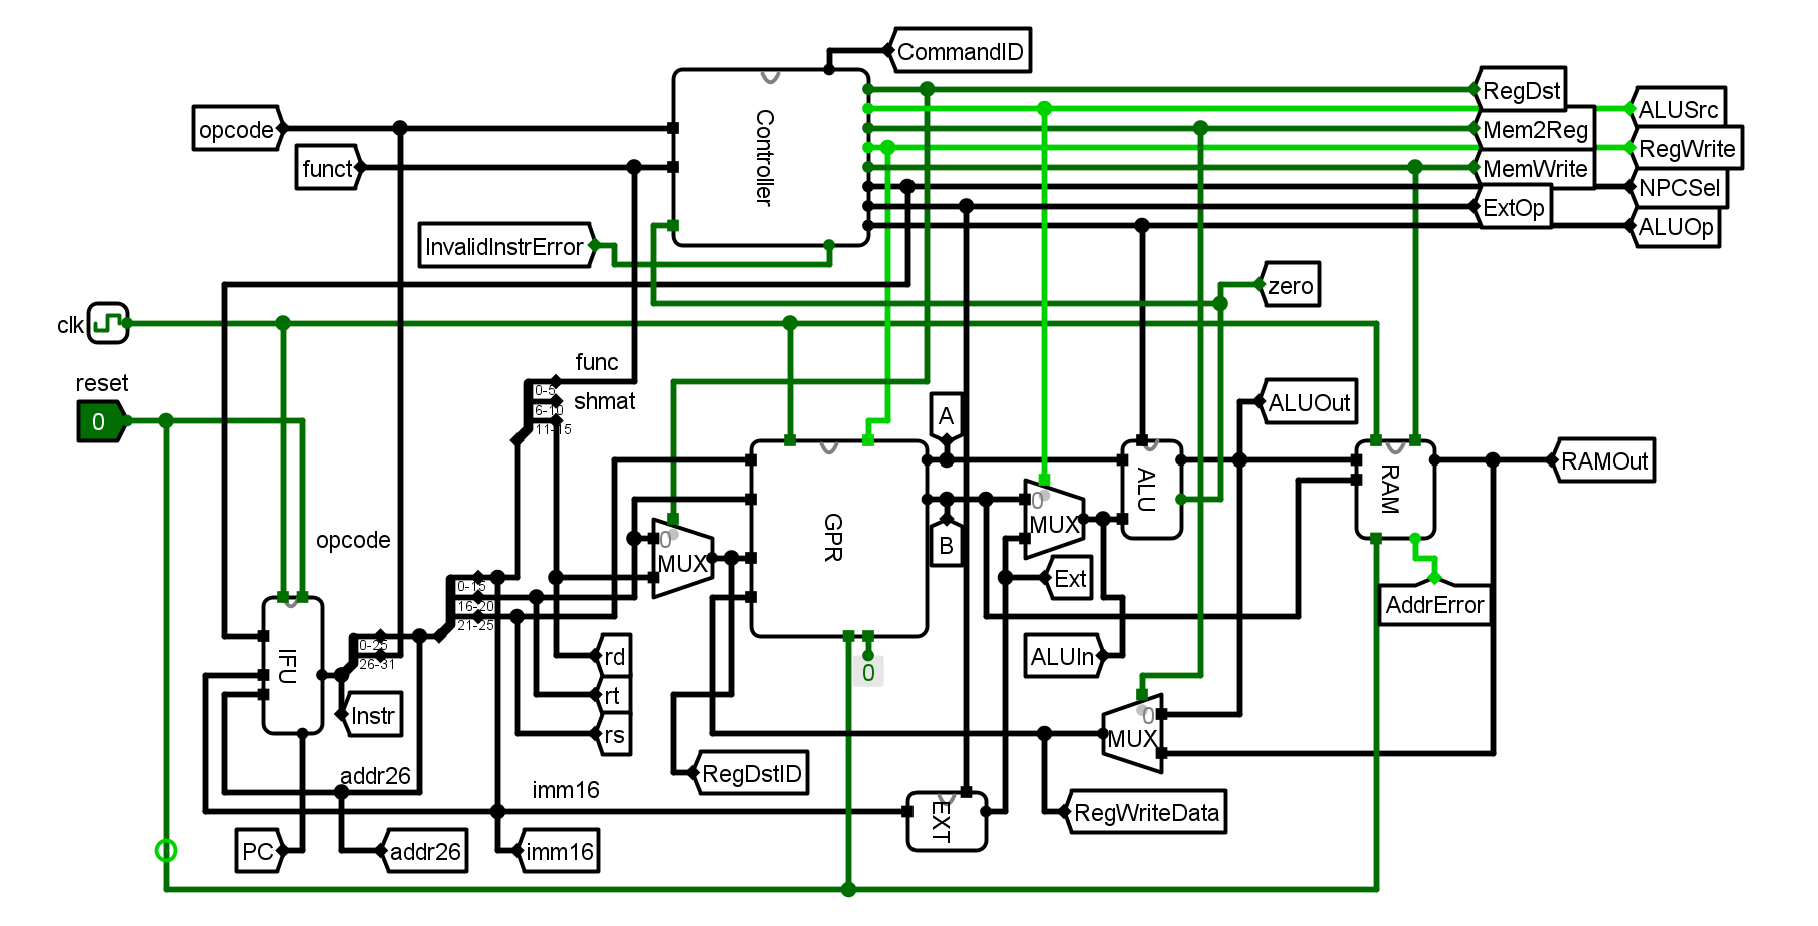
\includegraphics[width=\textwidth]{images/overall-circuit.png}
\caption{整体电路图}
\end{figure}

整体电路图中,标识了一些额外的信号,这主要是用于帮助调试可展示系统状态使用的,其具体功能如下表所示。

\begin{center}
    \captionof{table}{额外调试用信号}
    \begin{tabular}{c c c c}
        \toprule
        信号名称 & 信号类型 & 位宽 & 含义\\
        \midrule
        PC & 调试辅助信号 & 32bit & 程序计数器值 \\
        CommandID & 调试辅助信号 & 3bit & 指令类型编号 \\
        Inst & 调试辅助信号 & 32bit & 当前完整指令 \\
        RegDstID & MUX选择结果 & 5bit & 写入的寄存器编号 \\
        RegWriteData & MUX选择结果 & 32bit & 写入寄存器的数据 \\
        ALUIn & MUX选择结果 & 32bit & 输入ALU的第二个数据值 \\
        InvalidInstrError & 错误标识 & 1bit & 标识是否出现非法opcode \\
        AddrError & 错误标识 & 1bit & 标识是否出现内存地址未对齐4的倍数 \\
        \bottomrule
    \end{tabular}
\end{center}

这些额外信号的加入不会影响系统的功能,仅是为了帮助我们测试时了解系统的状态使用。
\end{document}
